\documentclass[include/preamble.tex]{subfiles}

% title information
\title{Coding by Shapes}
\subtitle{\texorpdfstring{$\square\bigtriangleup\bigtriangledown\bigcirc$}{}}
\author{Andy Scott}

\usenavigationsymbolstemplate{}

\begin{document}

%%%%%%%%%%%%%%%%%%%%%%%%

{
  \usebackgroundtemplate{
    
\includegraphics[width=\paperwidth]{images/bg_title.jpg}%
  }
  \frame{\titlepage}
}

{
  \usebackgroundtemplate{
    
\includegraphics[width=\paperwidth]{images/bg_coffee.jpg}
  }
  \begin{frame}
    \frametitle{who am I?}
    \begin{itemize}
      \pause
    \item contributor to a few Scala libs; maintainer of even fewer
    \item fan of graphs, trees, recursive structures
    \item also dogs, hiking, coffee, books, music
    \item work on Scala \& Bazel at Stripe
      \newline
      \pause
    \item \makebox[1.5cm]{github} \makebox[3.4cm]{https://github.com}/andyscott
    \item \makebox[1.5cm]{twitter} \makebox[3.4cm]{https://twitter.com}/andy$\cdot{g}\cdot$scott
    \end{itemize}
  \end{frame}
}

\tikzset{
  main node/.style={inner sep=0,outer sep=0},
  label node/.style={inner sep=0,outer ysep=.2em,outer xsep=.4em,font=\scriptsize,overlay},
  strike out/.style={shorten <=-.2em,shorten >=-.5em,overlay}
}

\newcommand<>{\acancelto}[3][]{
  \tikz[baseline=(N.base)]{
    \node[main node](N){$#2$};
    \node#4[label node, #1, anchor=south west] at (N.north east){\only#4{$#3$}};
    \draw#4[strike out,-latex,#1]  (N.south west) -- (N.north east);
  }
}

\begin{frame}
  \frametitle{Goals}
  \begin{itemize}
  \item learn some diagramming basics
    \pause
  \item code $\rightarrow$ diagrams
    \pause
  \item diagrams $\rightarrow$ code
    \pause
  \item keep it simple but cover useful concepts
  \end{itemize}
  \pause
  \hspace{3em}
  \begin{displayquote}
    the real treasure was the \acancelto<6->[red]{friends}{folds} we learned along the way
  \end{displayquote}
  \centerline{{\rm --- Jon Pretty}}
\end{frame}

\begin{frame}
  \begin{figure}
    \begin{center}
      \only<1>{\ldots}
      \only<2->{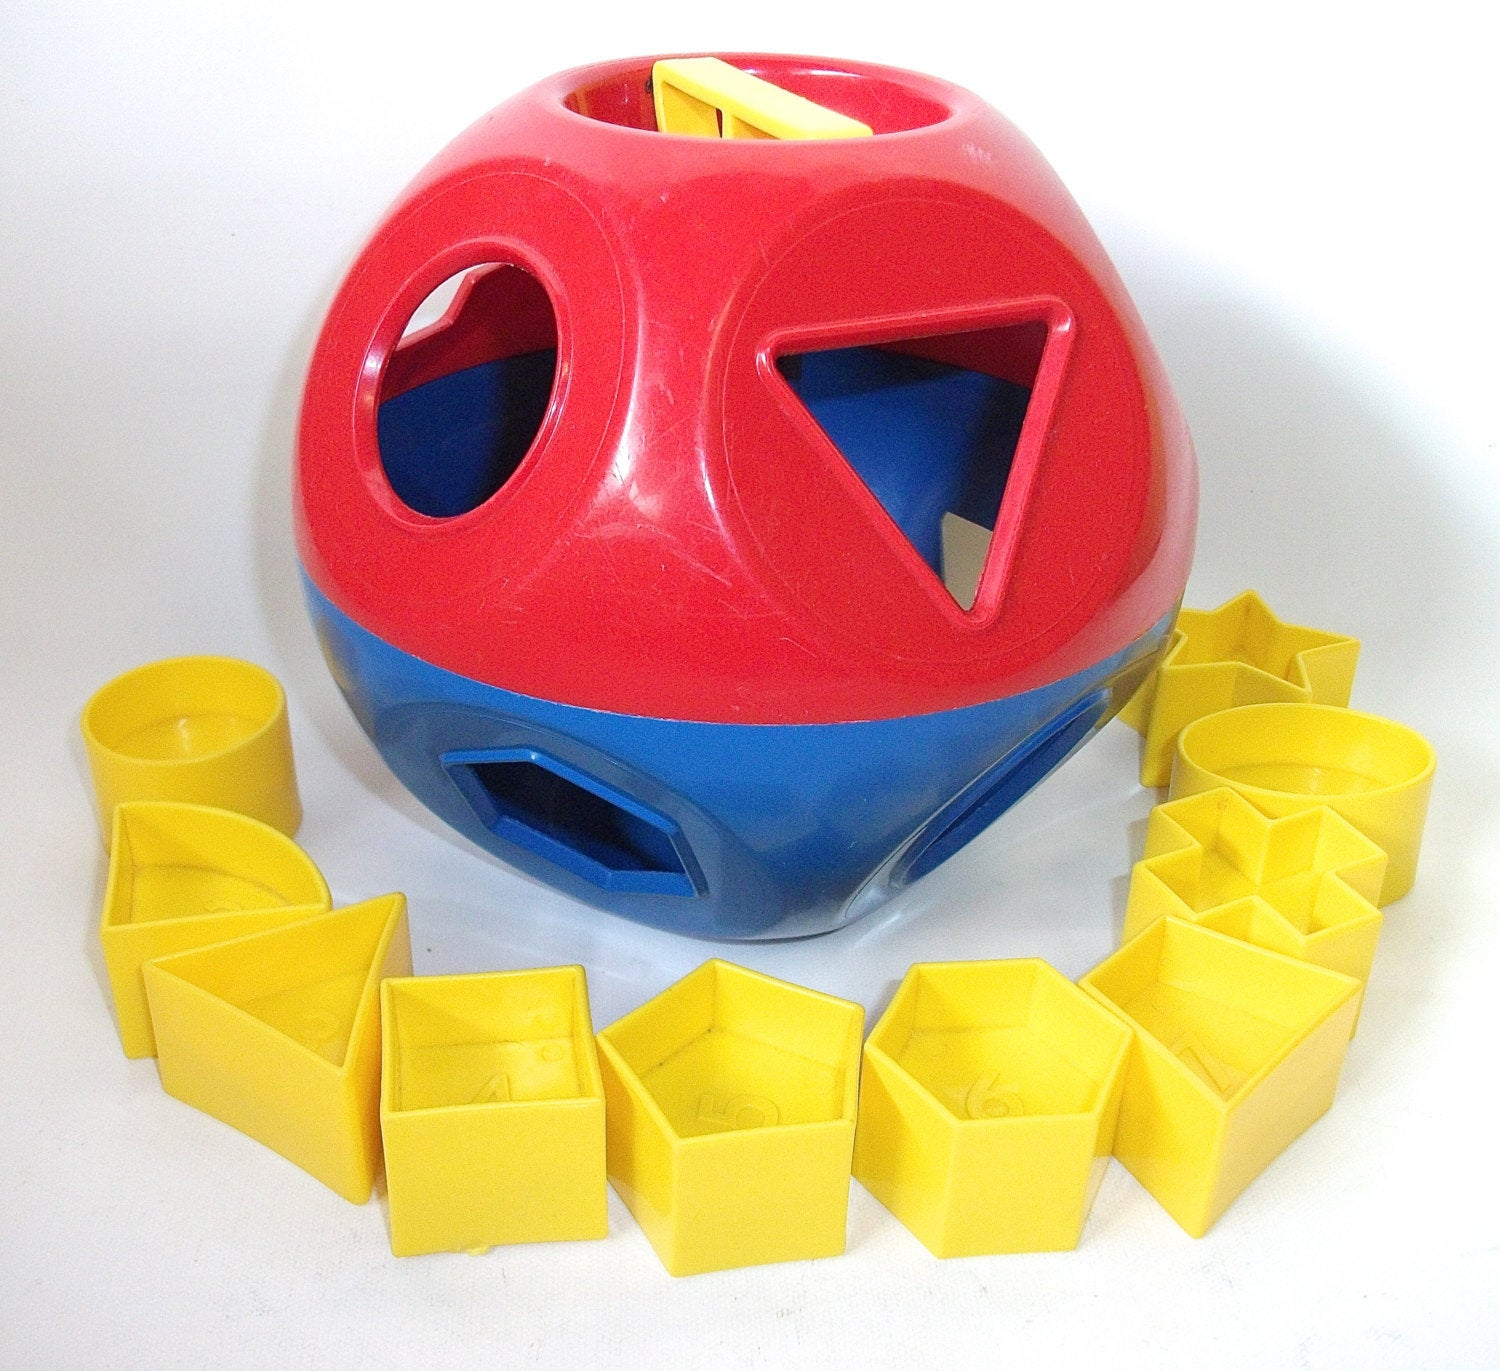
\includegraphics[width=0.6\textwidth]{images/tupperware-shape-o.jpg}}
    \end{center}
    \uncover<3->{\caption{Tupperware Shape-O}}
  \end{figure}
\end{frame}

{
  \usebackgroundtemplate{
    
\includegraphics[width=\paperwidth]{images/bg_coffee_blob.jpg}
  }

  \begin{frame}
    \frametitle{Commutative Diagram 101}
    \begin{itemize}
    \item it's a picture of composition
    \item nodes are objects
    \item edges are morphisms
    \end{itemize}
  \end{frame}

  \subfile{slide_world}
}

\begin{frame}[fragile]
  \begin{center}
    \begin{tikzcd}[matrix scale=2.5]
      A \arrow[rd, swap, "\only<2-4>{h}\only<6->{g \circ f}"] \arrow[r, "f"] & B \arrow[d, "g"] \\
      & C
    \end{tikzcd}
    \pause
    \pause
    \newline
    \newline
    \begin{lstlisting}[style=scala, escapeinside=||]
      def f(a: A): B = //...
      def g(b: B): C = //...
      def h(a: A): C = |\only<+>{???}\only<+>{g(???)}\only<+->{g(f(a))}|
    \end{lstlisting}
  \end{center}
\end{frame}

\section{examples}
\subsection{traverse}

\subfile{slide_traverse}
\subsection{hylo}

\subfile{slide_hylo}




%%%%%%%%%%%%%%%%%%%%%%%%%%%%%%%%%%%%%%%%%%%%%%%%

{
  \usebackgroundtemplate{
    
\includegraphics[width=\paperwidth]{images/bg_title.jpg}
  }
  \begin{frame}
    \begin{center}
      questions?
    \end{center}
  \end{frame}
}

%%%%%%%%%%%%%%%%%%%%%%%%%%%%%%%%%%%%%%%%%%%%%%%%
%%%%%%%%%%%%%%%%%%%%%%%%%%%%%%%%%%%%%%%%%%%%%%%%

\begin{comment}


\begin{frame}
  \begin{center}
    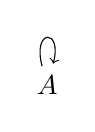
\begin{tikzpicture}
      \node {$A$} edge[loop above] (A);
    \end{tikzpicture}
  \end{center}
\end{frame}


\begin{frame}
  \frametitle{Visual Learning}
  \begin{displayquote}
    Visual learning is a style in which a learner
    utilizes graphs, charts, maps and diagrams.
  \end{displayquote}
  \rightline{{\rm --- Wikipedia}}
\end{frame}

\begin{frame}
  \frametitle{Categories}
  \begin{itemize}
  \item roughly: a collection of objects, with arrows between them
  \item restrictions
    \begin{itemize}
    \item identity arrow
    \item composition
    \end{itemize}
  \end{itemize}
\end{frame}

\end{comment}

\end{document}
